% =============================================================================
% SECCIÓN 2.2: TECNOLOGÍAS DESCENTRALIZADAS: BLOCKCHAIN
% =============================================================================
\section{Tecnologías Descentralizadas}

\subsection{Blockchain}
\label{sec:blockchain}

Blockchain es una tecnología descentralizada que utiliza una cadena de bloques enlazados criptográficamente para registrar transacciones de manera inmutable y distribuida. Esta estructura básica permite la verificación colectiva sin intermediarios confiables, estableciendo las bases para sistemas de consenso distribuido que garantizan la integridad de los datos mediante mecanismos criptográficos y protocolos de validación colectiva.

\subsubsection{Fundamentos de Blockchain}

Un blockchain consiste en una secuencia de bloques, donde cada bloque contiene un conjunto de transacciones válidas, una marca de tiempo, un número usado una única vez (nonce) y el resumen criptográfico (hash) del bloque anterior, lo que garantiza la inmutabilidad mediante la dependencia unidireccional de los resúmenes criptográficos. Esta estructura hace que cualquier modificación en un bloque propague cambios en todos los subsiguientes, detectándose fácilmente por la red distribuida \cite{nakamoto2008bitcoin, garay2015backbone}.

La arquitectura básica opera en una red peer-to-peer donde nodos mantienen copias completas del ledger, validando transacciones mediante funciones de resumen criptográfico (hash) como SHA-256 para enlazar bloques y prevenir alteraciones. La inmutabilidad surge de la dependencia unidireccional de los resúmenes criptográficos, haciendo el ledger resistente a manipulaciones retrospectivas una vez que un bloque alcanza suficiente profundidad en la cadena \cite{zheng2018blockchain, narayanan2016bitcoin}. Esta característica fundamental permite que blockchain funcione como un registro distribuido e inmutable, donde la confianza se establece mediante consenso algorítmico en lugar de autoridades centralizadas.

La Figura~\ref{fig:bloque_blockchain} ilustra la estructura básica de un bloque típico en una cadena blockchain, mostrando cómo cada bloque referencia criptográficamente al bloque anterior mediante su resumen criptográfico (hash), creando una cadena inmutable.

\begin{figure}[htbp]
    \centering
    \shorthandoff{>}
    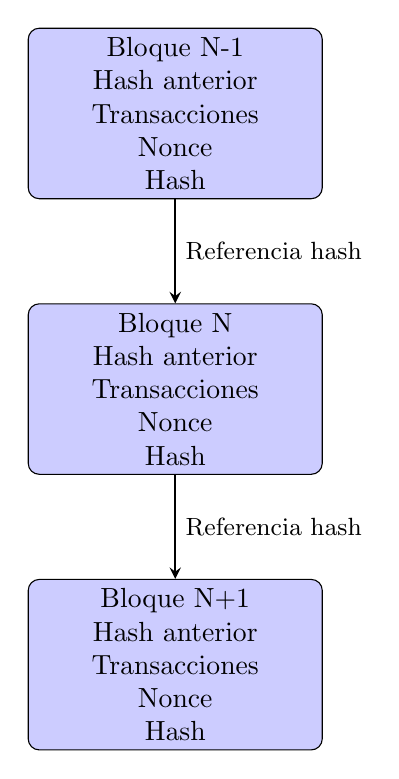
\begin{tikzpicture}[
        block/.style={rectangle, draw, fill=blue!20,
                      text width=3.5cm, text centered,
                      rounded corners, minimum height=2cm},
        arrow/.style={->,thick,>=stealth}
    ]
    
        % Bloques más separados verticalmente
        \node[block] (bloque1) at (0,7) {Bloque N-1 \\ Hash anterior \\ Transacciones \\ Nonce \\ Hash};
        \node[block] (bloque2) at (0,3.5) {Bloque N \\ Hash anterior \\ Transacciones \\ Nonce \\ Hash};
        \node[block] (bloque3) at (0,0) {Bloque N+1 \\ Hash anterior \\ Transacciones \\ Nonce \\ Hash};
    
        % Flechas largas con etiqueta pegada
        \draw[arrow] (bloque1.south) -- node[midway,right]{\small Referencia hash} (bloque2.north);
        \draw[arrow] (bloque2.south) -- node[midway,right]{\small Referencia hash} (bloque3.north);
    
    \end{tikzpicture}
    \shorthandon{>}
    \caption{Estructura básica de una cadena de bloques, mostrando la dependencia criptográfica entre bloques consecutivos.}
    \label{fig:bloque_blockchain}
    \end{figure}
    
    

\subsubsection{Arquitectura de Cadena Lineal}

Bitcoin y Ethereum ejemplifican arquitecturas de cadena lineal (o unidireccional), donde bloques se apendan secuencialmente formando una estructura cronológica irreversible. En Bitcoin, la cadena principal emerge del fork con mayor trabajo computacional acumulado (regla de la cadena más larga), mientras que Ethereum mantiene compatibilidad similar pero soporta estado mutable mediante contratos inteligentes ejecutables en una máquina virtual descentralizada \cite{nakamoto2008bitcoin, buterin2014ethereum}.

Esta linealidad asegura orden total en transacciones, diferenciándose de estructuras DAG (Directed Acyclic Graph) no lineales que permiten validación paralela. Bitcoin se enfoca principalmente en transferencias de valor, mientras que Ethereum extiende esta funcionalidad a contratos inteligentes y aplicaciones descentralizadas, ampliando significativamente las capacidades de la tecnología blockchain \cite{buterin2014ethereum, garay2015backbone}.

La arquitectura lineal presenta ventajas en términos de simplicidad y orden determinístico, pero introduce limitaciones en escalabilidad y throughput, ya que todas las transacciones deben procesarse secuencialmente en la cadena principal.

\subsubsection{Mecanismos de Consenso}

El consenso en blockchain resuelve el problema de acuerdo distribuido en entornos sin confianza, garantizando que todos los nodos honestos lleguen a un acuerdo sobre el estado del ledger. Los mecanismos de consenso más ampliamente adoptados son Proof-of-Work (PoW) y Proof-of-Stake (PoS), cada uno con características distintivas que equilibran seguridad, descentralización y eficiencia energética.

Proof-of-Work (PoW) requiere que los mineros compitan resolviendo puzzles computacionales complejos para proponer bloques válidos, asegurando que la cadena más larga represente la verdad aceptada por la mayoría de la potencia computacional de la red. Este mecanismo, implementado originalmente en Bitcoin, proporciona seguridad mediante el costo computacional requerido para modificar el historial, pero consume cantidades significativas de energía \cite{nakamoto2008bitcoin}.

Proof-of-Stake (PoS) selecciona propositores de bloques proporcionalmente a su participación económica (stake) en la moneda, reduciendo consumo energético al reemplazar trabajo computacional por compromiso económico. Ethereum adoptó PoS en su transición post-merge, logrando una reducción estimada del 99.9\% en consumo energético mientras mantiene propiedades de seguridad \cite{buterin2014ethereum}.

Ambos mecanismos conceptualmente priorizan liveness (progreso continuo de la cadena) y safety (consistencia del estado), tolerando hasta cierto umbral de nodos adversarios corruptos según el modelo de seguridad asumido. La Tabla~\ref{tab:pow_vs_pos} sintetiza las principales diferencias entre ambos mecanismos.

\begin{table}[htbp]
\renewcommand{\arraystretch}{1.3}
\caption{Comparación entre Proof-of-Work y Proof-of-Stake}
\label{tab:pow_vs_pos}
\centering
\footnotesize
\begin{tabular}{lcc}
\hline
\textbf{Criterio} & \textbf{Proof-of-Work (PoW)} & \textbf{Proof-of-Stake (PoS)} \\
\hline
Consumo energético & Alto (minería intensiva) & Bajo (validación ligera) \\
Velocidad de confirmación & Lenta (10 min Bitcoin) & Rápida (12 s Ethereum PoS) \\
Requisitos de hardware & Especializado (ASIC, GPU) & Estándar (servidores) \\
Seguridad & Basada en potencia computacional & Basada en stake económico \\
Descentralización & Alta (acceso abierto a minería) & Variable (requiere capital inicial) \\
Resistencia a ataques & 51\% de tasa de hash & 51\% de stake económico \\
Ejemplos & Bitcoin, Ethereum pre-merge & Ethereum post-merge, Cardano \\
\hline
\end{tabular}
\end{table}

\subsubsection{Limitaciones Principales}

Las blockchains lineales enfrentan limitaciones fundamentales que restringen su aplicabilidad en escenarios que requieren alto throughput, baja latencia o costos transaccionales reducidos. El trilema de escalabilidad (seguridad, descentralización, escalabilidad) establece que es difícil optimizar simultáneamente los tres aspectos, resultando en trade-offs inherentes \cite{zheng2018blockchain}.

El throughput limitado representa una restricción crítica: Bitcoin procesa aproximadamente 7 transacciones por segundo (TPS), mientras que Ethereum alcanza 20-30 TPS en condiciones normales, valores insuficientes para aplicaciones de alta frecuencia como sistemas de monitoreo urbano que requieren escritura frecuente de datos \cite{belotti2023scalability}. La latencia también constituye un desafío, con tiempos de bloque de 10 minutos en Bitcoin y 12 segundos en Ethereum, lo cual puede resultar inadecuado para aplicaciones que requieren confirmaciones rápidas.

Los costos transaccionales presentan variabilidad significativa, especialmente durante períodos de congestión de red. En Ethereum, los fees pueden oscilar entre \$0.50 y más de \$10 USD por transacción dependiendo del estado de la red, lo cual resulta prohibitivo para aplicaciones que requieren escritura frecuente de datos, como el reporte periódico de métricas de tráfico \cite{conoscenti2016blockchain, eckermann2021blockchain}.

La escalabilidad adicional se ve limitada por el crecimiento continuo del tamaño del ledger, que exige nodos completos con alto almacenamiento y ancho de banda, dificultando la participación de dispositivos con recursos limitados. Soluciones como sharding o capas secundarias (layer-2) mitigan parcialmente estos problemas pero introducen trade-offs en descentralización y complejidad operativa \cite{belotti2023scalability, zheng2018blockchain}.

Estas limitaciones motivan la exploración de arquitecturas alternativas, como BlockDAG, que ofrecen mejoras significativas en throughput, latencia y costos mediante estructuras no lineales que permiten procesamiento paralelo de transacciones.

